In this section, we discuss how to extend \textit{query split} to handle queries that contain other operations (e.g. outer join, semi join, or aggregation functions). We first give an overview of the extended \textit{query split} in Section 6.1, then introduce how to get the result of non-SPJ operations in Section 6.2. Although we have not implemented the support for these kinds of queries, the basic underlying ideas are quite straightforward. 
\subsection{Overview} \label{S61}
    To deal with non-SPJ queries, the basic idea is to split them into non-SPJ operations that connect several SPJ sub-queries and apply \textit{query split} on each sub-query.\par
    The workflow of the extended algorithm is shown in Figure \ref{F13}. If the query \textbf{Q} is a SPJ query, we simply run standard \textit{query split} on it. Otherwise, we process \textbf{Q} as follows:
    \begin{enumerate}[leftmargin = 15pt]
        \item We parse the query, and select a non-SPJ operator (denote as \textbf{op}) with maximal depth, such that all its inputs are SPJ queries.
        \item We obtain the result of \textbf{op} by the methods that we will describe in Section 6.2. 
        \item We generate a new query \textbf{Q'} from \textbf{Q} by regarding the result of \textbf{op} as a base relation.
        \item Repeat (1)-(3) on \textbf{Q'} until it becomes a SPJ query.
    \end{enumerate}
    \begin{figure}[htb]
        \centering
        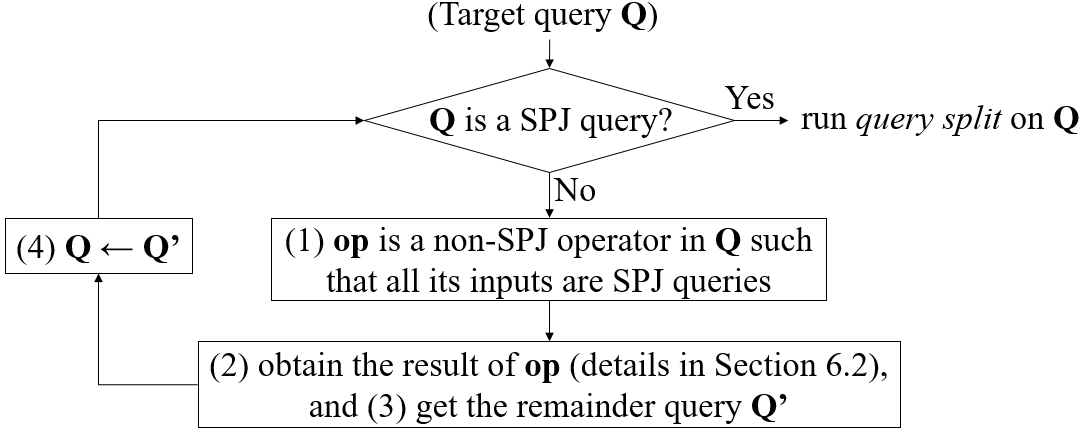
\includegraphics[width=\linewidth]{./pic/Figure13.png}
        \caption{The workflow of extended \textit{query split}}
        \label{F13}
        \Description{}
    \end{figure}

\subsection{Execute non-SPJ Operators} \label{S62}
    To obtain the result of a non-SPJ operator, we first construct the input sub-queries and execute them via \textit{query split}. Then, we deliver the sub-query results to the non-SPJ operator and execute it.\par
    As shown in Figure \ref{F14}, to deliver the sub-query results to the non-SPJ operator, we can choose either pipelining one tuple at a time or materializing the entire result. Note that this is different from standard \textit{query split}, since it is not necessary to gather run-time statistics. Although the run-time statistics can be used for choosing a better physical operator, the benefit of doing this is often very limited.
    \begin{figure}[htb]
        \centering
        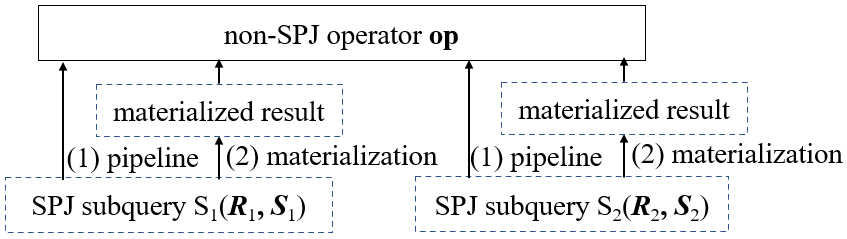
\includegraphics[width=\linewidth]{./pic/Figure14.png}
        \caption{Sub-queries of a non-SPJ operator}
        \label{F14}
        \Description{}
    \end{figure}